\documentclass[sim-use, blue_items]{checklist}
\usepackage{gensymb}
\usepackage{textcomp}

\logo{logo_white/boeing.png}
\title{Normal Procedures}
\subtitle{Boeing \\ 747-200}
\version{Version: 1.0 \\ \today}

\begin{document}

\begin{checklist}{Safety Check}
	\specialitem{Gear Lever}{Down}
	\specialitem{Flaps Lever}{In Same Position as Flaps themselves}
	\specialitem{Transponder}{Standby}
	\specialitem{Weather Radar}{Off}
	\specialitem{Galley Power}{All Off}
	\specialitem{Air Demand Hydraulic Pumps}{4 Off}
	\specialitem{Fuel Jettison Panel}{All Switches Off}
\end{checklist}

\begin{checklist}{Initial Powerup (Engineer)}
	\specialcondition{Establish Battery Power} {
		\item{Standby Power}{Off}
		\item{Main \& APU Battery DC Meters}{Check Voltage \& Amperage}
		\item{Battery}{On \& Guarded} 
	}
	\specialcondition{Establish External Power}{
		\item{External Power 1 \& 2 AC Meters}{Check Frequency \& Voltage}
		\item{External Power 1 \& 2 Connections}{Close}
	}
	\specialcondition{Standby Power} {
		\item{Standby Power}{Manual On}
		\item{Fuel Gauges \& Engine Instrument Flags}{Check On \& Off}
		\item{Standby Power}{Normal}
		\item{Fuel Gauges \& Engine Instrument Flags}{Check On \& Off}
	}
	\specialitem{Radio Master Bus} {Both On}
	\specialitem{APU Battery, Essential TR \& Battery DC Meters}{Check Positive Amperage}
	\specialcondition{Equipment Cooling Check} {
		\item{Equipment Cooling Smoke Detector Test}{Perform \& Check Light Illuminates}
		\item{Equipment Cooling Blower Test}{Perform \& Check Light Illuminates}
	}
\end{checklist}

\begin{checklist}{Pilot Panel Procedure (Engineer)}
	\specialitem{Engineer Panel Light Test}{Perform}
	\specialitem{Overhead Panel Light Test}{Perform}
\end{checklist}

\begin{continuedchecklist}
	\specialitem{Nav Lights} {On}
	\item{Logo Lights}{As desired}
	\item{No Smoking (\& Fasten Seatbelt) Signs}{On}
	\note{If the INS Systems have been shut off on through flights, the relevant steps have to be repeated.}
	\specialitem{INS 1, 2, 3}{Align}
	
	\specialcondition{INS Align (CIVA)} {
		\item{Status Page}{Check for Error Messages}
		\item{AUTO / MAN Switch}{Press to Test System}
		\item{Current Position}{Enter}
		\item{Before Continued Overhead Flow}{Wait until Status $\le$ 8}
		\note{Navigation is ready once status reaches 5.}
	}
	\specialcondition{Other INS / GPS Systems}{
		\item{Current Position}{Enter}
		\item{System}{Check for Errors}
		\item{Position Update System}{Set Up if possible \& desired}
	}
	
	\condition{Window Heat Tests} {
		\specialitem{Window Heat Power Lights}{On}
		\item{Window Heat}{4 On}
		\specialitem{Window Heat Overheat Test}{Press, Check Warning Light on Engineer Panel}
		\specialitem{Once Window Heat Lights Off}{Window Heat to Override, Check Lights On, Back To On}
		\specialitem{Window Heat Power Lights}{Off}
	}
	
	\specialcondition{Probe Heat Tests}{
		\item{TAT Test}{Left \& Right, Check TAT Probe Lights Extinguish}
		\item{Probe Heat}{Left \& Right On, Check All Lights Extinguish}
		\item{Probe Heat}{Left \& Right Off}
	}
	
	\condition{Warning Tests} {
		\item{Mach A/S Warning Test}{Test, Check Audio Warning}
		\item{Overrotation}{Test, Check Stick Shaker}
		\item{Stall Warning}{Test, Check Stick Shaker}
	}
	
	\condition{FO Side Overhead Flow} {
		\item{Engine 3 \& 4 Ignition}{Off}
		\item{FO Compass}{Slaved}
		\item{Altn Flap Selection}{Off}
		\item{FO HF}{Set to USB}
	}
	
	\item{Emergency Exit Lights}{On, Check Operation, Armed \& Guarded}
	\specialitem{Cockpit Voice Recorder}{Test, Check Double Bounce Of Needle}
	\specialitem{Wheel Well Fire Detection}{Test, Check Audible \& Visible Warning}
\end{continuedchecklist}

\begin{continuedchecklist}
	\condition{Capt Side Overhead Flow} {
		\item{Engine 1 \& 2 Ignition}{Off}
		\item{Capt Compass}{Slaved}
		\item{Altn Gear Extension}{Guard Closed}
		\item{SELCAL}{Set to HF1 \& HF2}
		\item{Capt HF}{Set to USB}
		\item{Body Gear Steering}{Armed \& Guard Open}
		\item{Anti Skid}{Guard \& Closed}
		\item{Autobrakes}{Off}
		\item{Flt Control Switches}{All Guarded}
	}
	\item{FDs \& WXR Radar Displays}{On for Both Pilots}
	\specialcondition{Pilot Panel Check}{
		\item{NAV Radio}{Tune any ILS Frequency, like 109.15}
		\item{UP/LT VOR Test}{Perform, Notice Needles Moving Up \& Left}
		\item{DN/RT VOR Test}{Perform, Notice Needles Moving Down \& Right}
		\item{Attitude Indicator Test}{Perform, Check Response}
		\item{Radar Altimeter Test}{Perform, Check Response \& Tone}
		\item{Autopilot Indicator Panel}{PTT 1 \& 2}
		\item{Instrument Selector Switches}{All Guarded}
		\item{Checks}{Repeat For FO}
	}
	\item{Max Indicators}{Reset}
	\specialitem{Altitude Alert Test}{Press, Reduce ALT SEL below current Altitude, Check Alert}
	\item{GPWS Test}{Perform, Check Alerts}
	\specialitem{Rudder Ratio Test}{Perform, Check Rudder Ratio Warning Light}
	\item{Instrument Warning Panels}{Reset}
	\item{Instrument Warning Test}{Perform, Check Lights}
	\item{Throttle 3}{Move Forward to Check Config Warning Horn}
	\item{Audio Panel}{Configure as Desired}
	\item{WXR Radar}{STBY, Tilt +5}
	\condition{Autothrottle Control Panel}{
		\specialitem{Test}{Perform at TOD \& CLB, Check EPR Limits on Main Panel increase}
		\item{EPRL Mode}{Set TOD}
	}
	\item{Rudder \& Aileron Trim}{Set 0}
\end{continuedchecklist}

\begin{checklist}{Engineer Panel Procedure (Engineer)}
	\condition{APU Powerup}{
		\item{APU Oil Quantity}{Check}
		\item{APU Power Selector}{On}
		\item{Boost Pump 2 Aft}{Check On}
		\specialitem{Squib Test}{Perform, Check Light}
		\specialitem{Fire Test A, B and Dual Check}{Perform, Check Alarm}
		\specialitem{Fault Test A, B}{Perform, Check Warning Light}
		\specialitem{Fault Test Dual}{Perform, Check Warning Light and Alarm}
		\item{APU}{Start}
		\item{APU Fields}{Close both Sides}
		\item{AC Meters}{Select \& Check APU Gen 1 \& 2}
		\item{APU Generators 1 \& 2}{Close}
	}
	\item{Galley Power}{On}
	\item{Galley Fan}{Auto}
	\item{Galley Chiller}{All On}
	\condition{If APU Air is not set up yet}{
		\item{Bleed Isolation Valves}{Close}
		\item{APU Bleed Air}{On}
		\item{Left Isolation Valve}{Open, Check Pressure > 30 PSI}
		\item{Right Isolation Valve}{Open, Check Pressure > 30 PSI}
	}
	\condition{Air Conditioning} {
		\item{PACK Controls}{All Auto}
		\item{PACK 1 and 3}{Open in sequence, check gauges for airflow}
		\item{Trim Air}{On}
		\item{Recirc \& Gasper Fans}{On as Desired}
	}
	\specialcondition{Cabin Pressurization Check}{
		\item{Mode Select}{Manual}
		\item{Outflow Valves Left \& Right}{Check Manual Close \& Open Fully}
		\item{Mode Select}{Auto}
		\item{Rate Limit}{Press, Check Warning Light \& Valves Close}
		\item{While Outflow Valves are still moving}{Manual Mode, Check Manual Control}
		\item{Mode Select}{Manual Left \& Right, Check Other Valve opens automatically, then Auto}
		\item{Rate Limit}{Press \& Release, Check Outflow Valves Open fully}
	}
	\item{Cabin Pressurization Mode Select}{Auto}
	\item{Cabin Pressurization Altitude}{Set Cruise Alt + 1000ft on Black Band, Set Standard QNH}
\end{checklist}

\begin{continuedchecklist}
	\specialcondition{Checks Upper Right Section} {
		\item{Squib Test Left \& Right}{Perform, Check Squib OK lights}
		\item{Fire \& Fault Test A \& B}{Perform, no Alarm}
		\item{Fire \& Fault Test Dual}{Perform, check Fire Lights \& Warning Bell}
		\item{Aft Cargo Heat}{Test, Check Lights}
		\item{Lower Cargo Fire Protection}{Test A \& B, check Warning Light, no Alarm}
		\item{Lower Cargo Fire Protection}{Test Dual, check Warning Light and Alarm}
		\item{Lower Cargo Fire Protection}{Test Squibs A \& B, check Lights}
		\item{Wing LE Overheat}{Test 1 \& 2, Check Lights}
	}
	\condition{Checks Right Section} {
		\specialitem{Brake Temp Monitor Test}{Activate, Check Light \& Gauges for all Sections High}
		\item{Brake Temp Monitor Test}{Deactivate, Check Gauges for all Sections Low}
		\specialitem{Data Recorder Lamp Test}{Perform, Check Lights}
		\specialitem{Anti Skid LDG Gear Tilt Input Test}{Perform Both, Check Light}
		\specialitem{Landing Gear Light Tests}{Perform all, Check Lights}
		\item{Potable Water}{Press to Read Gauge, Check Value}
		\specialitem{Hyd System Quantities}{Test, Check Needles \& Warning Lights}
		\item{Hyd System Quantities}{Check in green band}
	}
	\condition{Fuel System Checks}{
		\item{Block Fuel}{Crosscheck with Loaded Fuel}
		\item{Gross Weight Gauge}{Set}
		\specialitem{Fuel Gauge Test}{Test, Check Error 0, 4 and Segment Quantity Displays}
		\item{Fuel Used}{Reset}
		\specialitem{Fuel Heat}{All On then Off, check Open Lights turn on temporarily}
		\specialitem{Crossfeed Valves}{Toggle, Check Light, then Cycle back, check Light}
		\item{Crossfeed Valves}{Reserve, 2, 3 closed and 1 \& 4 open}
		\specialitem{Boost \& Ovrd Pumps}{All Fwd On, check FWD Pressure Lights turn off\\and AFT Pressure lights stay on, Pumps Off Again}
		\specialitem{Boost \& Ovrd Pumps}{All Aft On, check AFT Pressure Lights turn off\\and FWD Pressure lights stay on}
		\item{Boost \& Ovrd Pumps}{All On (Where Fuel in Tanks)}
	}
	\item{Oil Quantity \& Temp}{Check}
	\note{The engine oil quantity must be more than 3.5.}
\end{continuedchecklist}

\begin{checklist}{Preflight Preparations (Pilots)}
	\item{Relevant SID information}{Transfer Heading, NAV Frequencies and Courses to MCP}
	\item{MCP}{Confirm Heading Mode}
\end{checklist}

\begin{continuedchecklist}
	\item{MCP Nav Radio Mode}{Set if desired depending on first used VOR and Course}
	\item{Cleared Altitude / First Stop Altitude}{Set on MCP}
	\item{Altitude Select}{Activate}
	\item{QNH}{Set on Pilot and Standby Altimeters}
	\item{Waypoints}{Enter in all Navigation Systems \& Crosscheck}
	\item{INS Align Switches}{NAV once fully aligned}
	\item{Transponder Code}{Set}
	\item{Performance Calculations}{Calculate, Set Bugs}
	\item{Stab Trim Green Band}{Change if necessary}
	\item{Initial Pitch}{Set On FD}
	\item{EPRL Mode}{Verify TOD}
	\item{Aileron \& Rudder Trim}{Verify Zero}
\end{continuedchecklist}

\begin{checklist}{Pushback \& Engine Start Preparations}
	\item{Brake Pressure}{Check in Green Band}
	\condition{If Brake Pressure too low}{
		\item{Electric Hydraulic Pump (System 4)}{On}
		\item{Brake Pressure}{Check Increase to Green Band}
	}
	\item{Bleed Valves}{Open}
	\item{Parking Brake}{Check Set}
	\item{Ground Equipment}{Remove}
	\item{Before Start Checklists}{Perform}
	\condition{Before Start Checklist Considerations} {
		\item{Flight Director}{Manually Check, Takeoff with FD on}
		% \item{Bleed Controls}{Skip, Leave PACKs on while on Stand}
		\item{EPR Computer}{Manually Check, Takeoff in TOD Mode}
		\item{Air Conditioning Controls}{Skip, Leave PACKs on while on Stand}
	}
	\condition{Hydraulic Pressurization} {
		\item{Wait For}{Hydraulic Pressurization OK}
		\item{Air Hydraulic Pump 1}{On}
		\item{Electric Hydraulic Pump (System 4)}{On}
	}
	\item{Fuel Pumps}{Check All On}
	\item{Engine Oil Quantities}{Check}
\end{checklist}

\begin{checklist}{Pushback}
	\item{Transponder}{XPDR}
	\item{Pushback Clearance}{Received}
	\item{INS 1, 2, 3}{Verify NAV}
	\item{Beacon Light}{On}
	\item{Seatbelts and No Smoking Signs}{Verify On}
	\item{Body Gear Steering}{Verify Armed}
	\item{One PACK}{Switch Off (One is still on)}
	\item{Electrical Panel}{Check}
	\item{Galley Power}{Switch Off}
	\item{Hydraulic Pressure 1 \& 4}{Verify}
	\item{Pushback}{Start}
	\note{End pushback with straight segment to straighten Body Gear Steering.}
\end{checklist}

\begin{checklist}{Engine Start}
	\item{All PACKs}{Switch Off}
	\item{Before Start Checklist}{Go over Skipped Items}
	\item{Fuel Pumps}{Check All On}
	\item{Engine Oil Quantities}{Check}
	\item{Engine Bleed Valves}{Check Open}
	\item{Duct Pressure}{Check Sufficient}
	\item{Start Valve}{ARM}
	\condition{Repeat for Engine 4, 1, 2, 3} {
		\item{Engine Ignition 1 or 2}{Ground Start until Starter Valve Open}
		\item{N2}{Check Increasing}
		\item{Oil Pressure}{Check Increasing}
		\item{At 20\% N2}{Fuel On}
		\note{Use Rich instead of Idle if the EGT is lower than 0 $^\circ C$, then Idle after stabilized.}
		\item{EGT}{Check Increase}
		\item{N1}{Check Acceleration}
		\item{Once Starter trips Off}{Start Next Engine}
	}
\end{checklist}

\begin{checklist}{After Start Procedure}
	\item{Start Valve}{Off \& Guarded}
\end{checklist}

\begin{continuedchecklist}
	\item{Probe Heaters}{On}
	\item{APU Bleed}{Off}
	\condition{Transfer Electric Source}{
		\item{Generators}{Check Operation On AC Meter, then close Connection}
		\item{Split System Breaker}{Close}
		\item{Galley Power}{All On}
	}
	\item{PACKs}{All On}
	\item{Air Pumps}{All On}
	\item{Electric Hydraulic Pump}{Check Off, Close Guard}
	\item{Aft Cargo Heat}{Normal}
	\item{Flaps}{Select}
	\item{Stab Trim}{Set}
	\item{Aileron \& Rudder Trim}{Check Zero}
	\item{Flight Control Check}{Perform}
	\item{After Start Checklist}{Perform}
	\item{APU}{Switch Off 2 Minutes after Pneumatic Operation}
	\item{Taxi Checklist}{Perform}
\end{continuedchecklist}

\begin{checklist}{Taxi}
	\condition{After Leaving Ramp} {
		\item{Autothrottle Mode}{EPR}
		\item{EPRL Mode}{Check TOD}
		\item{Weather Radar Mode}{WXR}
		\item{Transponder}{TA/RA}
		\item{Cabin Crew}{Notify For Takeoff}
	}
	\condition{Before Runway Entry} {
		\item{All PACKs}{Switch Off}
		\item{Ignition Switches}{All Flight Start}
		\item{Landing Lights}{On}
		\item{Runway Turnoff Lights}{Off}
		\item{Strobe Lights}{On}
		\item{Before Takeoff Checklist}{Perform, Skip Body Gear Steering}
	}
	\condition{After Lineup}{
		\item{Gear Not Centred Lights}{Check Off}
		\item{Body Gear Steering}{Off, Close Guard}
	}
\end{checklist}

\begin{checklist}{Takeoff}
	\item{Manually Apply Thrust}{Until Stabilized}
	\item{Elapsed Timer}{Start}
	\item{Autothrust}{On}
	\item{Autothrottle EPR Indication}{Check On}
	\note{To prevent a tail strike, keep pitch below 10° before positive rate is achieved.}
	\item{Initial Pitch}{Maintain V2 to V2 + 15,\\In 4-Engine Climbout set Lower End of Pitchbar "L" to selected Pitch}
\end{checklist}

\begin{checklist}{Initial Climb}
	\note{A flap setting can be used if the speed is at or above the respective bug.\\Limit turns to 15° until V2 + 100 is reached.\\When flying close (< 10 - 15 nm) to a VOR, don't use this VOR for VOR/LOC. Switch to heading mode instead.}
	\item{Close In Turns $\leq$ 25°}{Fly in Takeoff Config if necessary}
	\item{Thrust Reduction Height (1500ft)}{Wait For}
	\item{EPRL Mode}{CLB}
	\note{Reducing thrust to CLB can be delayed until Flaps 5 are set if a steeper climb is required.}
	\condition{Flaps 20 Takeoff} {
		\item{Flaps 10 Speed}{Accelerate To}
		\item{Flaps 10}{Set}
	}
	\item{At Acceleration Height (immediately or 3000ft)}{Accelerate to\\Restriction, 250 kts or Climb Speed}
	\condition{Cleanup} {
		\item{Gear Lever}{Off}
		\item{Ignition}{Turn Off}
		\item{Landing Lights}{Turn Off Half}
		\item{PACKs}{All On}
		\item{Fuel Config}{Adjust}
		\item{Fuel Heat}{Auto}
	}
	\item{When Levelling Off}{Set Altitude Hold}
	\condition{Passing Transition Altitude}{
		\itemcustcase{Altimeter}{SET STANDARD PRESSURE 29.92 inHg / 1013 hPa}
	}
\end{checklist}

\begin{continuedchecklist}
	\condition{Passing 10000ft} {
		\item{Best Climb Speed}{Accelerate To}
		\item{All Landing \& Logo Lights}{Off}
		\item{Humidifier}{On}
		\item{Seatbelt Signs}{Off If Desired}
		\item{After Takeoff Checklist}{Perform}
	}
\end{continuedchecklist}

\begin{checklist}{Cruise}
	\condition{At TOC} {
		\item{EPRL Mode}{CRZ}
		\item{Air Conditioning System}{Reconfigure for Cruise}
	}
	\item{INS Waypoints}{Update if Necessary}
	\item{Fuel Config}{Adjust when Necessary}
\end{checklist}

\begin{checklist}{Descent \& STAR Planning}
	\item{Destination Airport}{Set as Waypoint in INS, use as Distance Indicator}
	\condition{Switch to Radio Nav if necessary} {
		\item{Frequencies \& Courses}{Set}
		\item{MCP Nav Radio Mode}{Set if desired depending on first used VOR and Course}
		\item{HSI Display Selector}{Select Radio}
		\item{Heading Bug}{Set to aid VOR Course interception}
		\item{MCP}{Select Heading, then VOR}
	}
	\item{If using INS for STAR}{Start DME/DME Updates}
	\condition{Calculate TOD} {
		\note{If the altitude difference between restrictions times 3 is greater than the distance between them, the later restriction is stricter.}
		\note{Start the descent 1 nm earlier for every 10 kts that the plane has to slow down.}
		\item{Determine Distance to Restriction}{Multiply Altitude to Descent in 1000ft times 3}
		\item{Start Descent}{When Distance to Restricting Waypoint Approaches Calculation}
		\note{The required rate of descent is the current ground speed $\cdot$ 5.}
	}
	\item{Minimums}{Set on Barometric / Radar Altimeter}
	\item{Landing Performance}{Calculate Speeds, Set Autobrake}
	\item{Note Clean Speed}{F1 + 20}
\end{checklist}

\begin{checklist}{Top of Descent}
	\item{Altitude Bug}{Set cleared Altitude or first Restriction}
	\item{Descent}{Start, Stay at current Speed until 10000ft}
	\item{Cabin Pressurization Altitude}{Set Landing Alt on White Band, Set Destination QNH}
	\item{Fuel Heat}{Off}
	\item{Reserve Fuel Valves}{Open}
	\item{Air Conditioning System}{Reconfigure for Descent}
	\condition{Passing 10000ft}{
		\item{Half of the Landing Lights}{Turn On}
		\item{Logo Lights}{On If Desired}
		\item{Seatbelt Signs}{Check On}
		\item{EPRL Mode}{Go Around}
		\item{Humidifier}{Off}
		\item{Descent \& Approach Checklist}{Perform, Skip Radio/INS Switches if necessary}
	}
	\condition{Passing Transition Level} {
		\item{Altimeter}{Set Pressure at Destination Airport}
	}
\end{checklist}

\begin{checklist}{Approach}
	\item{At roughly 25 nm}{Decelerate to clean Speed}
	\condition{For Radio Approaches}{
		\item{MCP Nav Radio Mode}{Dual}
	}
	\item{Until 15 nm}{Decelerate to Flaps 10}
	\item{Until 10 nm}{Set Flaps 20}
	\item{Until 8 nm}{Gear Down, Flaps 20 Speed}
	\item{Until 5 nm}{Landing Flaps \& Speed}
	\item{Ignition Switches}{All Flight Start}
	\item{All Lights}{On}
	\item{Speed Brake}{Arm}
	\item{Cabin Crew}{Notify For Landing}
	\item{Landing Checklist}{Perform}
	\condition{Once On Glidepath} {
		\item{Missed Approach Altitude}{Set}
	}
	\item{At 50 ft}{Retard Thrust Levers}
	\item{At 30 ft}{Flare}
\end{checklist}

\begin{checklist}{Go Around}
	\item{Go Around Button}{Press}
	\item{Go Around Thrust}{Set or activate Autothrust}
	\item{Pitch \& Speed}{Achieve 12$^\circ$, Hold Vref + 10, use Pitch Bar}
	\item{Flaps}{Set 20}
	\condition{Once Positive Rate}{
		\item{Gear}{Up}
	}
	\item{MCP}{Select Heading or as desired}
	\item{Altitude Select}{Activate}
	\item{Autothrust}{Manually activate Speed Mode or Set Speed bug to Clean Speed}
	\item{Clean Up}{Via After Takeoff Procedure}
\end{checklist}

\begin{checklist}{After Landing \& Taxi}
	\item{Body Gear Steering}{Arm}
	\condition{Cleanup}{
		\item{Reversers}{Stow}
		\item{Autobrake}{Off}
		\item{Flaps}{Up}
		\item{Speedbrake}{Retract}
		\item{Landing Lights}{Off}
	}
	\condition{After leaving Runway}{
		\item{Strobe Lights}{Off}
		\item{Probe Heat \& Anti Ice}{Off}
		\item{Ignition}{Off}
		\item{FDs}{Off}
		\item{Stabilizer Trim}{Set 7}
		\item{Transponder}{XPDR}
		\item{Weather Radar}{Stby}
		\item{Weather Radar Tilt}{+0}
		\item{Pressurization Mode Select}{MAN}
		\item{Outflow Valves}{Open Manually if Necessary}
		\item{Aft Cargo Heat}{Off}	
	}
	\item{After Landing Checklist}{Perform}
	\item{APU Power Selector}{On}
\end{checklist}

\begin{continuedchecklist}
	\condition{When entering Ramp}{
		\item{APU}{Start}
	}
	\condition{Before Turning Onto Stand} {
		\item{Runway Turnoff Lights}{Off}
	}
\end{continuedchecklist}

\begin{checklist}{Parking}
	\item{Parking Brake}{Set}
	\item{Split System Breaker}{Open}
	\item{APU Fields}{Close both Sides}
	\item{AC Meters}{Select \& Check APU Gen 1 \& 2}
	\item{APU Generators 1 \& 2}{Close}
	\item{Engines}{Shut Down}
	\item{Transponder}{Stby}
	\condition{After Engines have spooled down}{
		\item{Beacon Lights}{Off}
	}
	\item{Ground Connections}{Establish}
	\item{Unloading}{Begin}
	\note{If the APU isn't used for electric power or bleed air, it can be shut off now.}
	\condition{Once Chocks are in Place}{
		\item{Parking Brake}{Disengage}
	}
	\item{ADPs}{Off}
	\item{Fuel Pumps}{Off}
	\item{Reserve Valves}{Close}
	\condition{If APU Bleed desired}{
		\item{PACK 2}{Close}
		\item{APU Bleed Air}{On}
	}
	\condition{Else} {
		\item{All PACK Valves}{Close}
	}
	\item{Window Heat}{Off}
	\item{INS}{Check Accuracy, Realign for Through Flight or shut off}
	\item{Secure Cockpit Checklist}{Perform To Line, Check Brakes (and INS) Manually}
\end{checklist}

\begin{checklist}{Shutdown}
	\specialitem{Emergency Lights \& No Smoking Signs}{Off}
\end{checklist}

\begin{continuedchecklist}
	\specialitem{INS \& Radio Master Switches}{Off}
	\specialitem{WXR Radar Display}{Off}
	\specialitem{Weather Radar}{Off}
	\specialitem{PACKS}{All Closed}
	\specialitem{Bleed Valves}{All Closed}
	\specialitem{Recirc Fans}{Off}
	\specialitem{Gasper Fans \& Trim Air}{Off}
	\specialitem{Ground Power \& APU Generators}{Disconnect}
	\specialcondition{If APU Running}{
		\item{APU Bleed}{Off}
		\item{APU}{Switch Off 2 Minutes after Pneumatic Operation}
	}
	\specialcondition{Shutdown Remaining Systems}{
		\item{Galley Power}{Off}
		\item{Galley Fan}{Off}
		\item{Galley Chiller}{All Off}
		\item{Standby Power}{Off}
	}
	\specialitem{Secure Cockpit Checklist}{Finish}
	\specialitem{Battery}{Off after APU Inlet Door Closed}
\end{continuedchecklist}

\begin{figure}[ht]
    \centering
	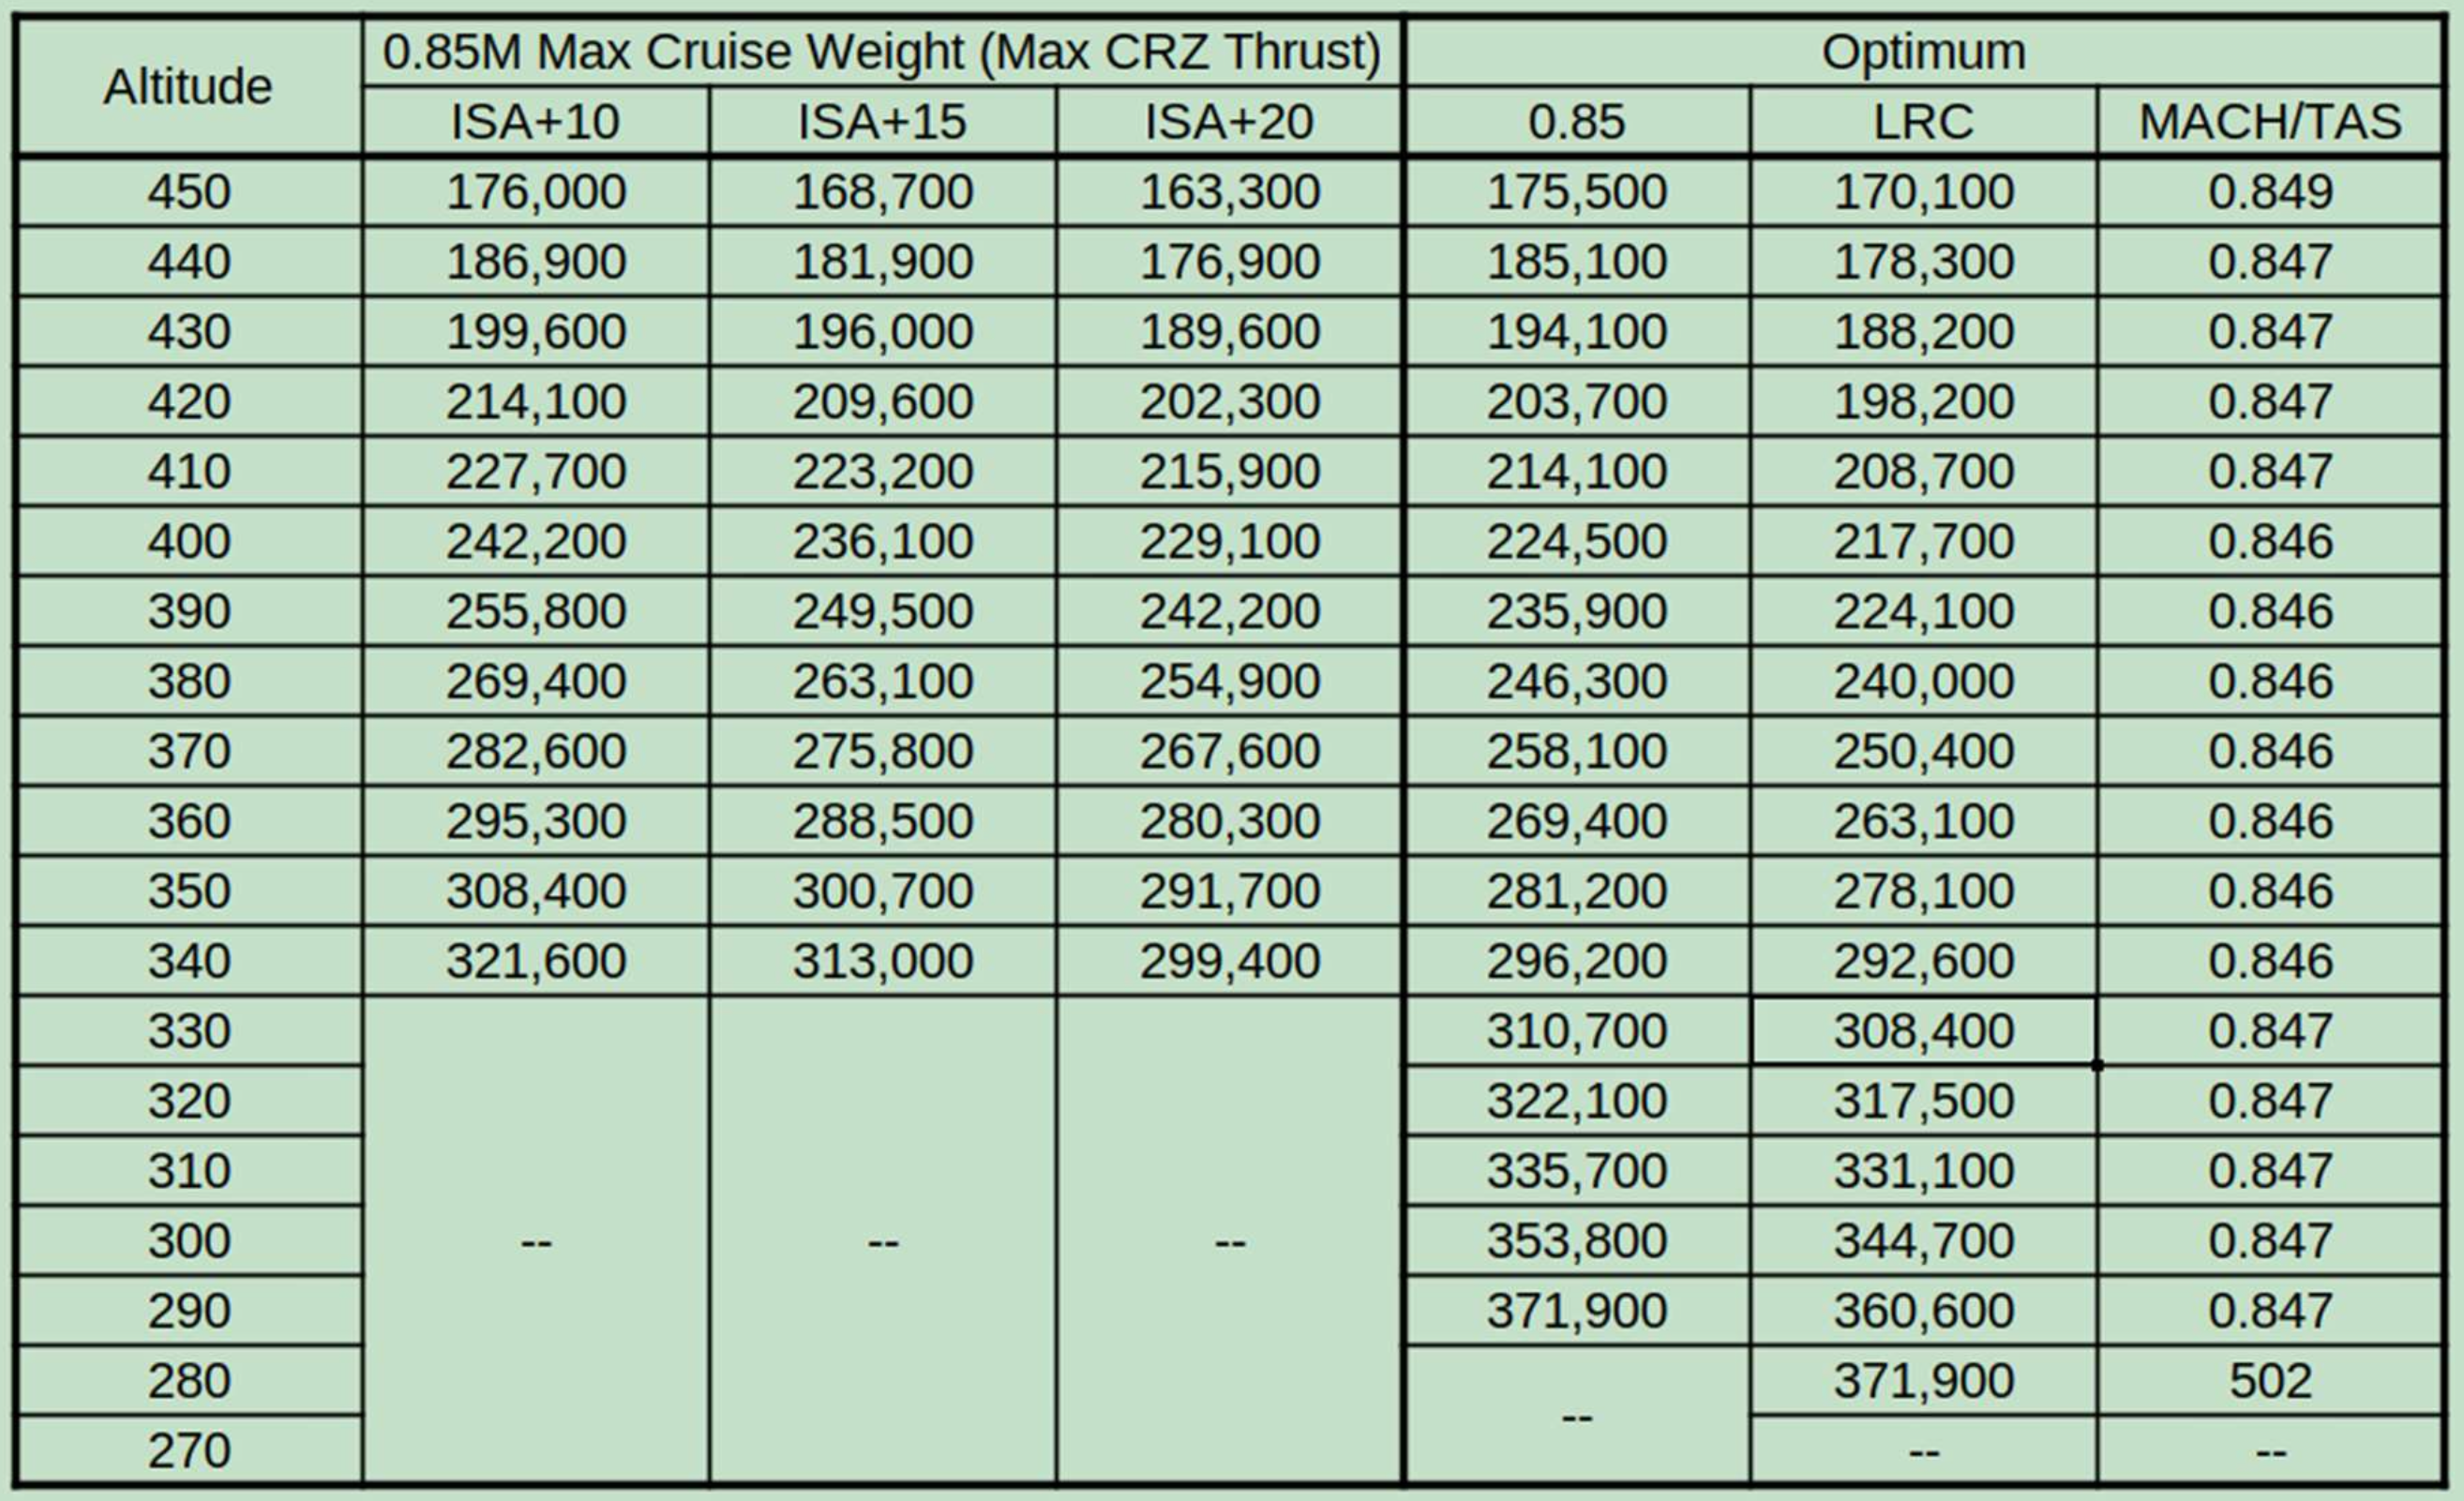
\includegraphics[width=\linewidth]{addenda/maxaltitude_kg_felis.png}
    \caption{Maximum \& Optimum Cruise Altitudes for Gross Weights in Kilogram,\\ISA Temp. at Sea Level: $15^\circ C$, $-2^\circ C$ per 1000ft}
\end{figure}

\begin{figure}[ht]
    \centering
	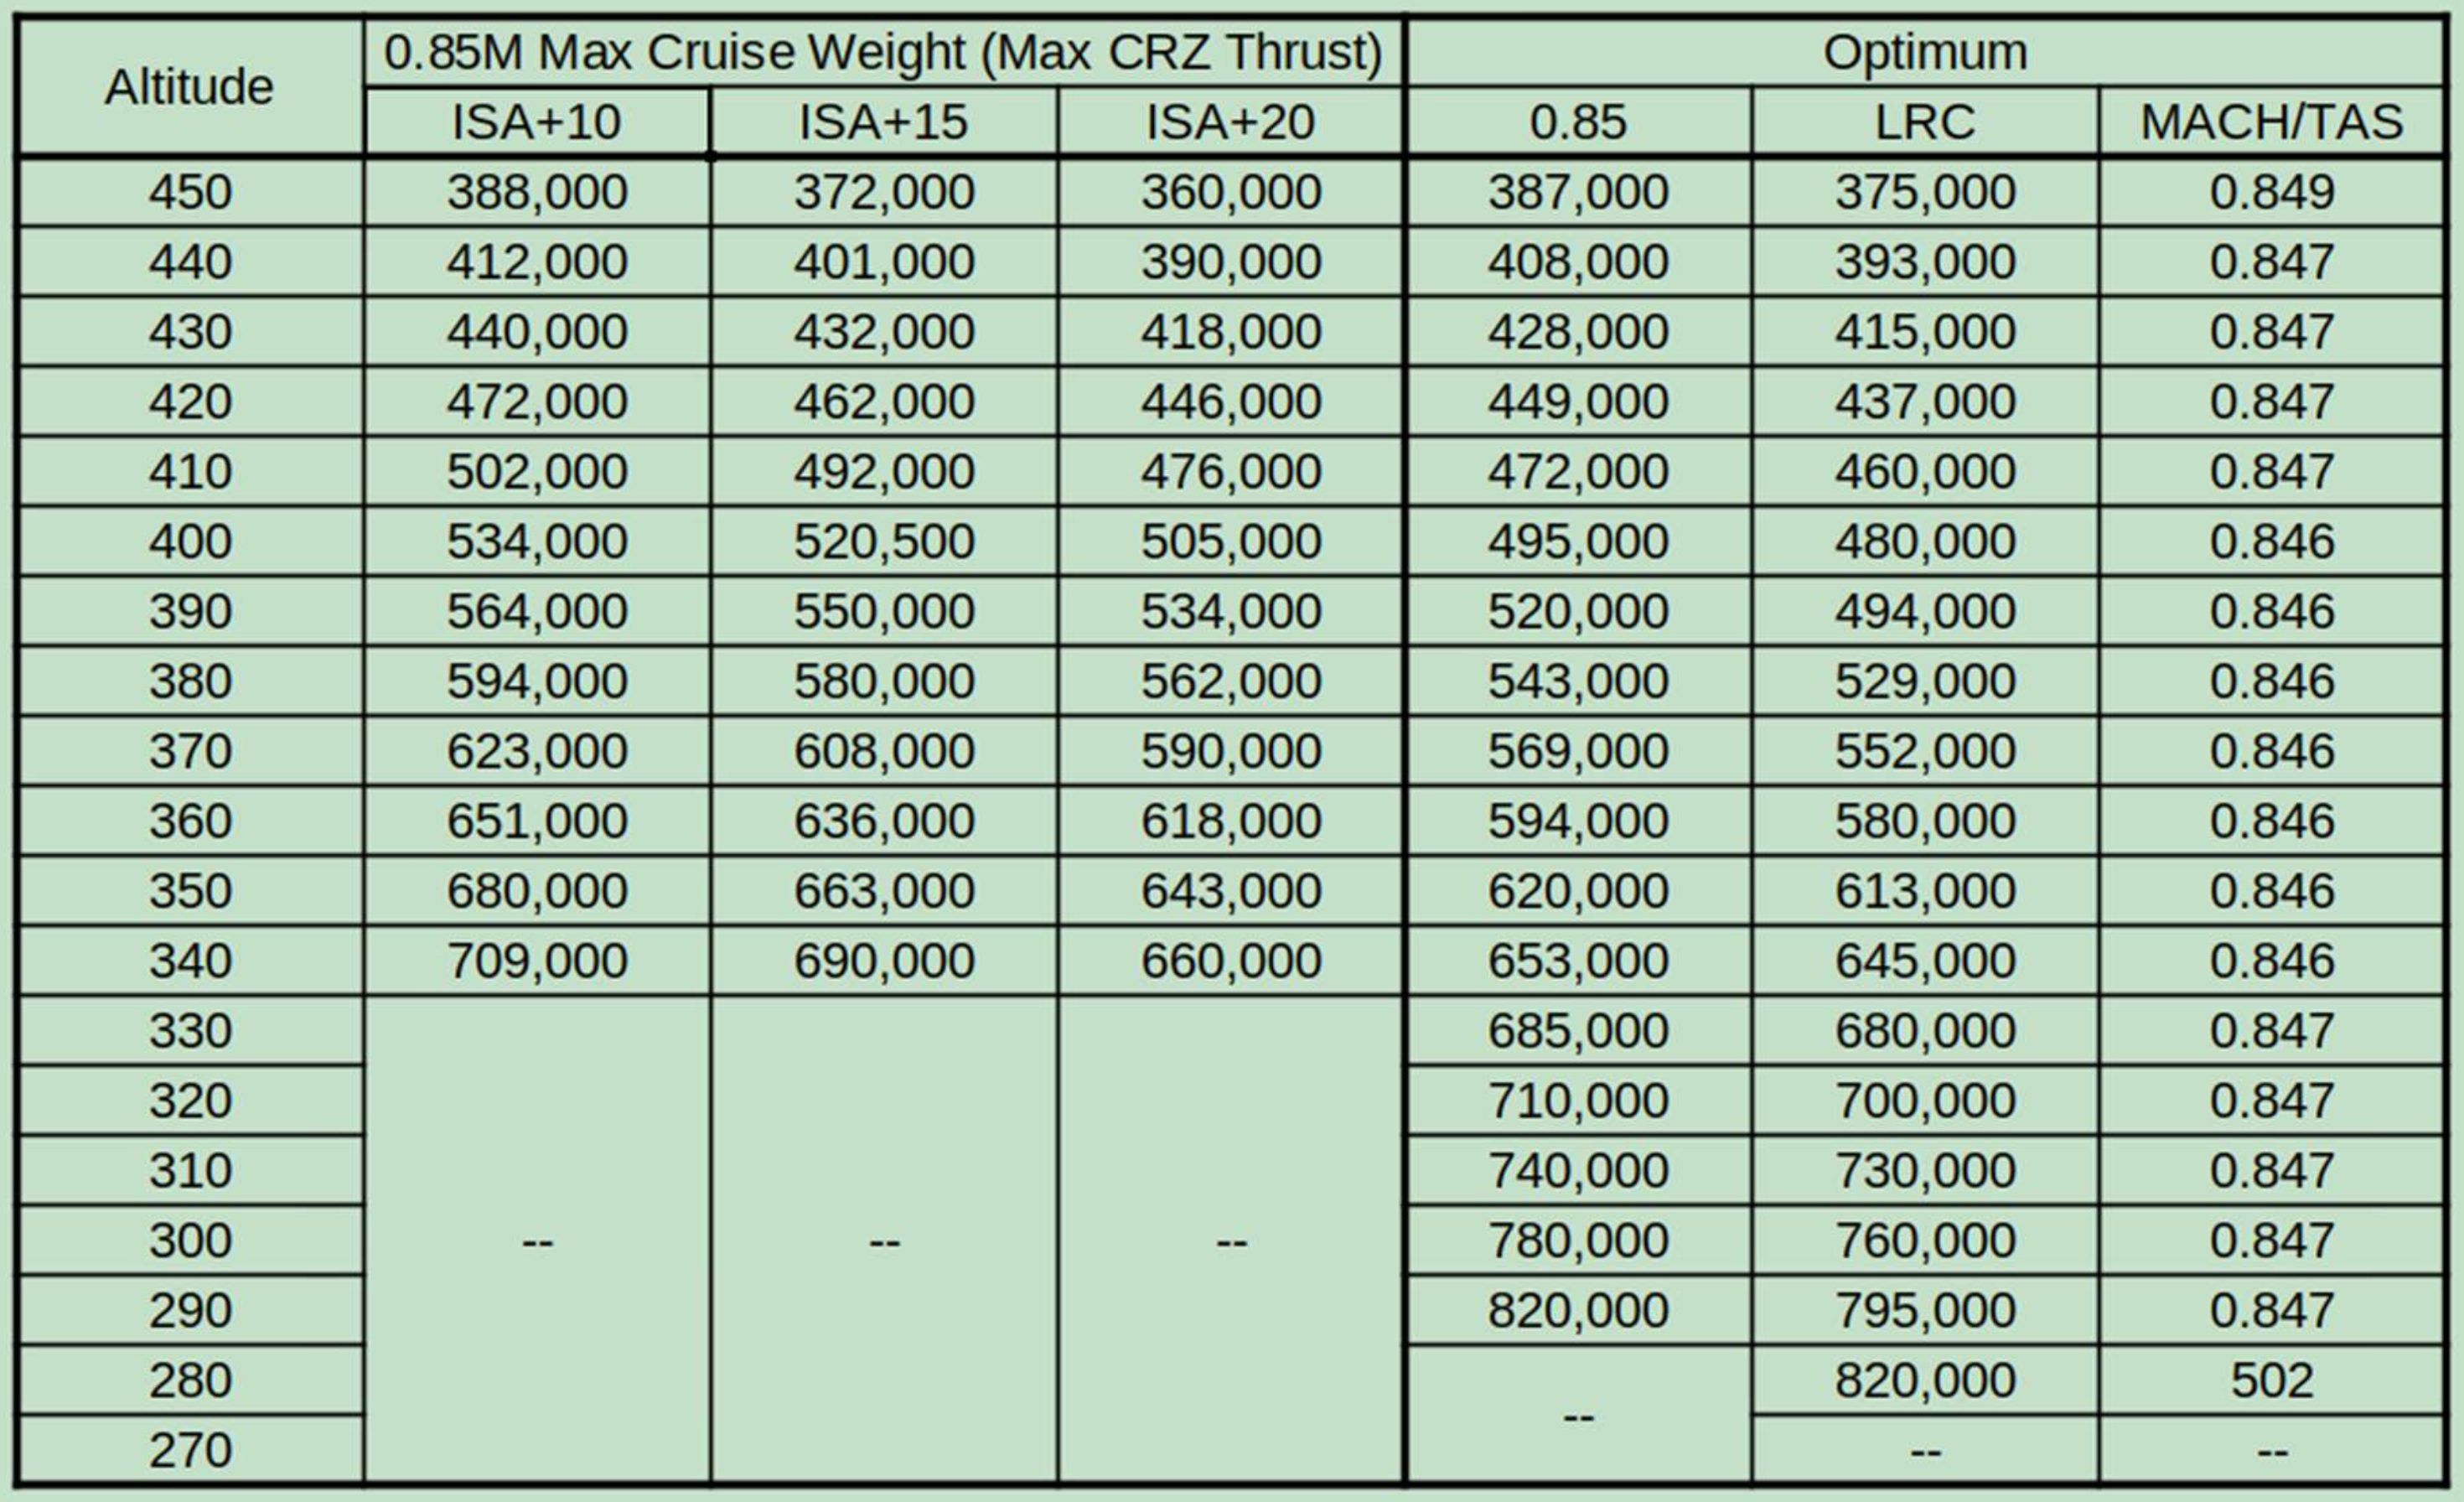
\includegraphics[width=\linewidth]{addenda/maxaltitude_lb_felis.png}
    \caption{Maximum \& Optimum Cruise Altitudes for Gross Weights in Pounds,\\ISA Temp. at Sea Level: $15^\circ C$, $-2^\circ C$ per 1000ft}
\end{figure}

\begin{figure}[ht]
    \centering
	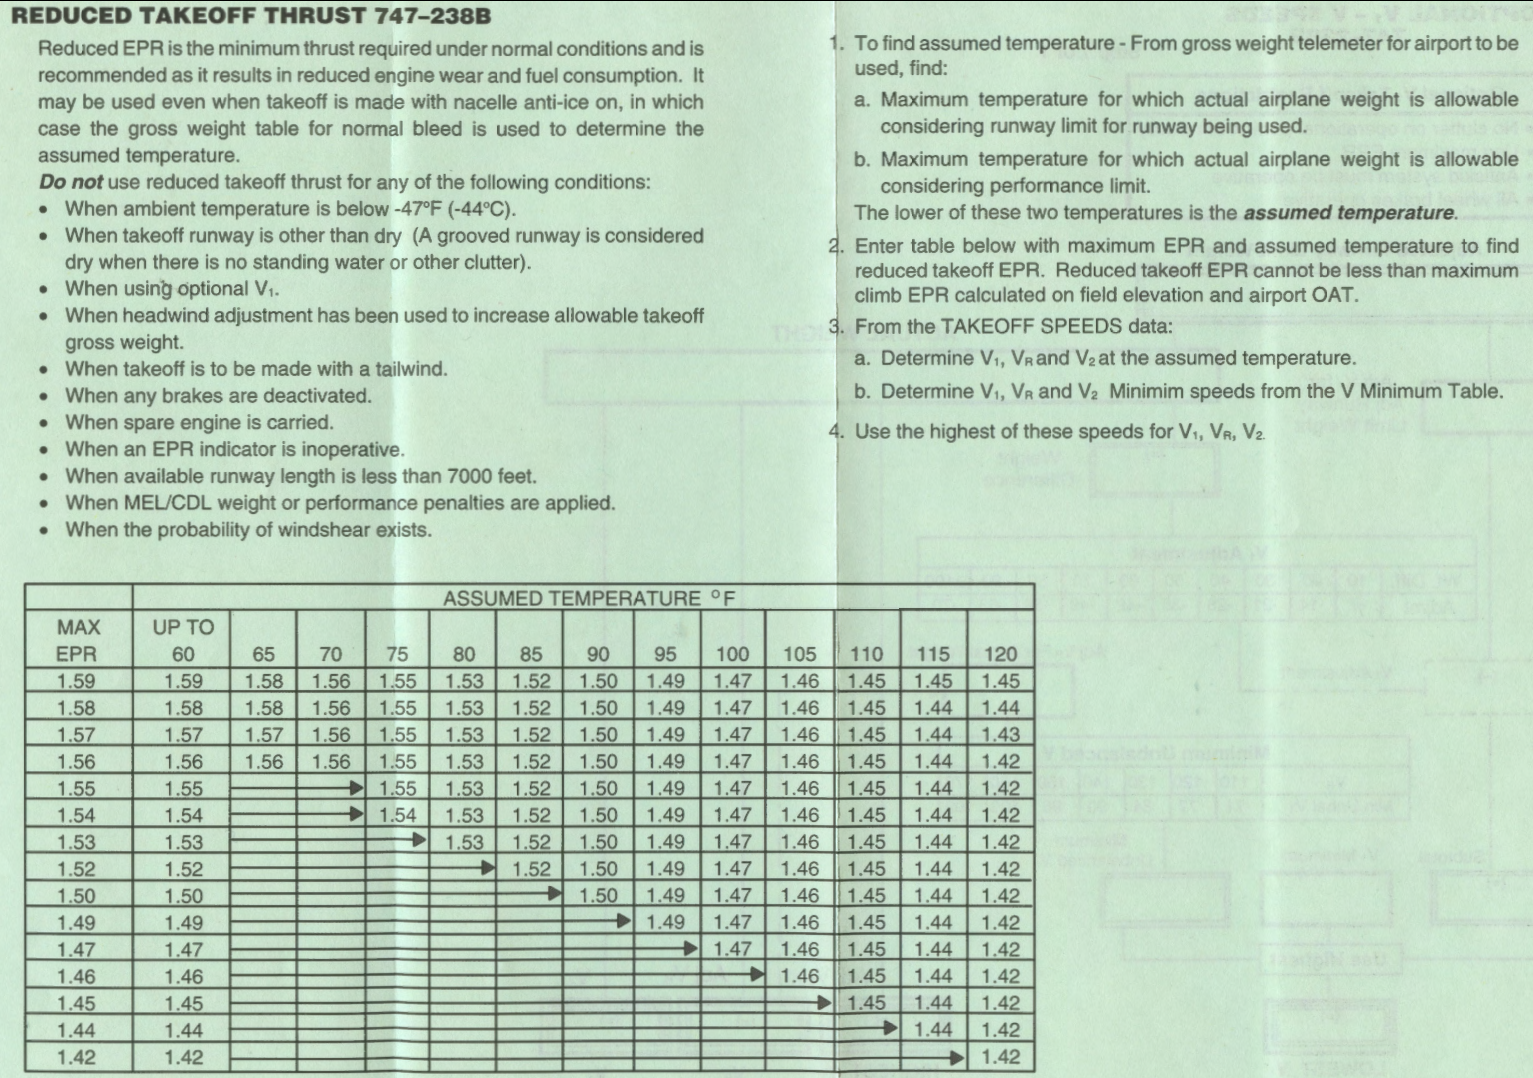
\includegraphics[width=\linewidth]{addenda/assumed_temp_742.png}
    \caption{EPR from Assumed Temperature, $^\circ F =\ ^\circ C \cdot 1.8 + 32$}
\end{figure}

\end{document}